\chapter{Calculations}
	\label{ch:calculations}

	This chapter explains:
	\begin{itemize}
    \item how to format numbers for convenient display;
    \item how to use the mathematical library functions;
    \item how to carry out both business and scientific calculations.
	\end{itemize}


  \section{Introduction}
	We have already seen in \Cref{ch:var} how to carry out simple calculations. This chapter is about more serious calculations. It enhances the earlier explanation and brings together all the information needed to write programs that carry out calculations. If you are not interested in programs that do numerical calculations, skip this chapter.
		
		Calculations arise in many programs – not just programs that carry out mathematical, scientific or engineering calculations. In information systems, calculations arise in payrolls, accountancy and forecasting. In graphics, calculations are necessary to scale and move images on the screen.

		\Cref{ch:var} explained several important ideas about numbers and calculations. The reader might like to review that chapter before continuing. The ideas were:
		\begin{itemize}
      \item input and output using text boxes and labels;
      \item conversion between the string representations of numbers and their internal representations;
      \item precedence rules in expressions;
      \item conversions in expressions that mix \keyword{Integer} and \keyword{Double} data.
		\end{itemize}


	\section{Literals}
		A value like 10 000 or 12.34 is named a \emph{literal} in the jargon of programming languages. If the programmer uses a literal such as 10000, the compiler assumes that the number is an \keyword{Integer}. If a value like 12.34 is used in a VB program, it is assumed by the compiler to be a \keyword{Double} value.
		
		Very large or very small \keyword{Double} literals can be written using exponent notation:
		\begin{itemize}
			\item 0.0001 is the same as \keyword{1.0E-4}
			\item 12300000.0 is the same as \keyword{1.23E7}
		\end{itemize}
		where for example \keyword{E4} means × 104.
		
		\begin{stqb}
			\begin{STQ}
			\item	Write these quantities as literals in exponent form:
				\begin{lstlisting}
5000
-0.00000056
				\end{lstlisting}
			\end{STQ}
		\end{stqb}


	\section{Formatting numbers}
	Formatting is the setting out of text in a convenient way. The display of numbers is especially important, as we do not want them to be misinterpreted. Also we don't always need the detail of unnecessary decimal places. For example, if the value \keyword{33.198765} represents the area of a room in square metres, then all the decimal places are probably not necessary.
		
	VB has a large range of facilities for formatting values, but here we restrict ourselves to the most common cases of formatting \keyword{Integer} and \keyword{Double} values. Each data type has a \keyword{Format} method, to which we can pass two parameters:
		\begin{itemize}
      \item a value to be formatted, and
      \item a string containing format information.
		\end{itemize}
		The method returns a string containing the formatted value, which is ready to be displayed.
		
		We will start out with \keyword{Integer} values. Suppose we have an integer value:
		\begin{lstlisting}
Dim i as Integer = 123
		\end{lstlisting}
		We have already widely used the \keyword{CStr} method to convert a number:
		\begin{lstlisting}
Label1.Text = CStr(i)
		\end{lstlisting}
		which gives the string:
		\begin{lstlisting}
123
		\end{lstlisting}
		But now we will use the formatting method \keyword{Format}. For example:
		\begin{lstlisting}
Dim formattedValue as String
Dim i as Integer = 123
formattedValue = Format(i, "0000")
Label1.Text = formattedValue
		\end{lstlisting}
		This causes the label to be given the value:
		\begin{lstlisting}
0123
		\end{lstlisting}
		because a zero in a format string means that a digit will always be produced at the position indicated. We would use this format string when we know that the integer may be up to four digits long, and we want to align the numbers in a tabular form.
		
		Another formatting character is the \# character. This stipulates that a digit will only appear when needed. For example:
		\begin{lstlisting}
Label1.Text = Format(123, "#####")
		\end{lstlisting}
gives the string:
		\begin{lstlisting}
123
		\end{lstlisting}
		For large integer numbers, commas can make the number more readable. This is illustrated by the following code:
		\begin{lstlisting}
Label1.Text = Format(123456, "#,###,###")
		\end{lstlisting}
		which gives the string:
		\begin{lstlisting}
123,456
		\end{lstlisting}
		Formatting tends to be more useful when \keyword{Double} values are to be displayed. The same formatting characters (\#, 0 and comma) are used, with the addition of the period character to specify where the decimal point is to be placed. In this example:
		\begin{lstlisting}
Dim formattedValue as String
Dim d as Double = 123.456
FormattedValue = Format(d, "0.00")
Label2.Text = formattedValue
		\end{lstlisting}
		the label is assigned the value:
		\begin{lstlisting}
123.46
		\end{lstlisting}
		On the left of the decimal point, digits are displayed as needed to present all of the number. But at least one digit is displayed. On the right of the decimal point, the number is rounded in order to fit into the two digits specified.
The following table gives a summary of the special characters in format strings.

		\begin{center}
			\begin{tabular}{lp{10cm}}
				\toprule
				.	& Place the decimal point here.\\
				0	& Place a digit here. If the data value is too small and does not fill the format, a 0 is inserted.\\
				\#	& Place a digit here, but if the value does not fill the format, nothing is displayed – not even a space.\\
				, &	Place a comma here.\\ \bottomrule
			\end{tabular}
		\end{center}

		\begin{stqb}
			\begin{STQ}
			\item What do these give:
				\begin{lstlisting}
Label1.Text = Format(0.123, "0.00")
Label1.Text = Format(123456.7, "#,###,###.00")	
				\end{lstlisting}
			\end{STQ}
		\end{stqb}


	\section{Library mathematical functions and constants}
		It is common in mathematical, scientific or engineering programs to use functions like sine, cosine and log. In VB, these are provided in one of the libraries – the \keyword{Math} library. To use one of the functions, you can write, for example:
		\begin{lstlisting}
x = Math.Sqrt(y)
		\end{lstlisting}
		Alternatively you can use an Imports statement at the top of the program like this:
		\begin{lstlisting}
Imports System.Math
		\end{lstlisting}
		and then write the more concise:
		\begin{lstlisting}
x = Sqrt(y)
		\end{lstlisting}
		Some of the more widely used functions in the \keyword{Math} library are given in alphabetical order below. Where the parameter is an angle, it must be expressed in radians.

		\begin{center}
			\begin{tabular}{>{\collectcell\keyword}l<{\endcollectcell} p{12cm}}
				\toprule
				Abs(x) & the absolute value of \keyword{x}, sometimes written $|x|$ in mathematics\\
				Ceil(x) & rounds \keyword{x} up to the smallest \keyword{Integer} greater than or equal to \keyword{x}\\
				Cos(x) & cosine of the angle \keyword{x}, where \keyword{x} is expressed in radians\\
				Exp(x) & $e^x$\\
				Floor(x) & rounds \keyword{x} down to the smallest \keyword{Integer} less than or equal to \keyword{x}\\
				Log(x) & natural logarithm of \keyword{x} (to the base $e$)\\
				Log10(x) & logarithm to base 10 of \keyword{x}\\
				Max(x,y) & the larger of \keyword{x} and \keyword{y}\\
				Min(x,y) & the smaller of \keyword{x} and \keyword{y}\\
				Pow(x,y) & \keyword{x} raised to the power of \keyword{y}, or $x^y$\\
				Round(x) & rounds a \keyword{Double} value to the nearest \keyword{Integer} value; for example \keyword{Math.Round(3.4)} is 3.0 – with a decimal point\\
				Sin(x) & sine of the angle \keyword{x}, expressed in radians\\
				Sqrt(x) & the positive square root of \keyword{x}\\
				Tan(x) & tangent of the angle \keyword{x}, expressed in radians\\\bottomrule
			\end{tabular}
		\end{center}

		When you use these methods, you sometimes have to be careful about the type of the variables or literals used as parameters. For example, the method \keyword{Abs} can be passed any numeric values but the method \keyword{Cos} can only be passed a \keyword{Double} number.
		
		The mathematical constants pi ($\pi$) and $e$ are also available as properties within the \keyword{Math} library, so that we can write, for example:
		\begin{lstlisting}
Dim x, y As Double
x = Math.PI
y = Math.E
		\end{lstlisting}
		or you can use an \keyword{Import} statement:
		\begin{lstlisting}
Imports System.Math
and then write:
x = PI
z = E
		\end{lstlisting}


	\section{Constants}
		Constants are values that don't change while the program is running. We have already met two, \keyword{E} and \keyword{PI}, that are already provided for use in the \keyword{Math} class. But it is often the case that there are other values in a program that will not change. Examples could be the factor for converting inches to centimetres, or the velocity of light. One approach is to write the values for these quantities directly into the program, like this:
		\begin{lstlisting}
cm = inches * 2.54
		\end{lstlisting}
		Another, better, approach is to declare such numbers as variables that have a constant value and give them a name, for example:
		\begin{lstlisting}
Const inchesToCm As Double = 2.54
		\end{lstlisting}
		A variable declared like this cannot be changed (by an assignment, for example) when the program runs. In fact the compiler will reject any attempt made to give such a variable a new value. We can then use the name in the calculation:
		\begin{lstlisting}
cm = inches * inchesToCm
		\end{lstlisting}
		This is clearer because we are using the programming language to explain what we are doing, rather than using unexplained numbers.

		\begin{stqb}
			\begin{STQ}
				\item The velocity of light is 299 792 458 metres per second. Write this as a \keyword{Double} constant.
			\end{STQ}
		\end{stqb}

		
	\section{Case study – money}
		We will now trace the development of a program to carry out calculations with money. In most countries, money comes in two parts – dollars and cents, euros and cents, pounds and pence. We have a choice – we can represent an amount of money either as a \keyword{Double} quantity (like 20.25 dollars) or as an \keyword{Integer} (2025 cents). If we use cents, we will need to convert amounts into dollars and cents and vice versa. We will opt to use \keyword{Double} variables to represent values.
		
		We will construct a program that calculates compound interest. An amount is invested at a particular annual interest rate and accumulates in value. The user enters the initial amount (as a whole number) and an interest rate (a number that may have a decimal point) into text boxes. The user then clicks on a button to see the amount accumulated each year, as shown in \Vref{fig:calculations_money_screen}. We start by declaring the main quantities:
		\begin{lstlisting}
Dim rate, newAmount As Double
Dim oldAmount As Double
		\end{lstlisting}
		\begin{figure}[bth]
			\centering
			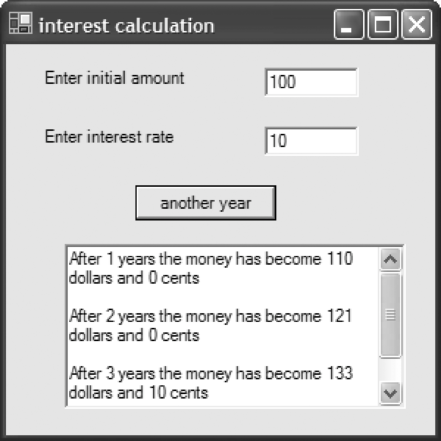
\includegraphics[width=8cm]{calculations_money_screen}
			\caption{Screen display of interest calculation.}
			\label{fig:calculations_money_screen}
		\end{figure}


		When the button is clicked to move on to the next year, the program must calculate:
		\begin{lstlisting}
newAmount = oldAmount + (oldAmount * rate / 100)
		\end{lstlisting}
		When we display an amount of money, we need to display a whole number of dollars and a whole number of cents, so that if the value is 127.2341 dollars for example, we need to display it as 127 dollars and 23 cents.
		
		First the dollar part. Simple use of the cast operator \keyword{CInt} converts the \keyword{Double} number to an \keyword{Integer}, truncating the fractional part:
		\begin{lstlisting}
dollars = CInt(newAmount)
		\end{lstlisting}
		Next the cents part. We need to get rid of the dollars part of the number. We can do this by subtracting the whole number of dollars so that a number like 127.2341 will become 0.2341. Now multiply by 100.0 to convert to cents, so that 0.2341 becomes 23.41. Next use \keyword{Math.Round} to convert to the nearest whole number (23.0). Then finally we convert the \keyword{Double} value to an \keyword{Integer} value using \keyword{CInt}.
		\begin{lstlisting}
cents = CInt(Math.Round(100 * (newAmount – dollars)))
		\end{lstlisting}
		We can now display the values properly converted. Finally,
		\begin{lstlisting}
oldAmount = newAmount
		\end{lstlisting}
		which is what investment is all about.
		
		The complete program follows and the form is shown in Figure 12.1. At the class level, the instance declarations are:
		\begin{lstlisting}
Private year As Integer = 1
Private oldAmount As Double
The response to a button-click is:
Private Sub Button1_Click( sender As System.Object,
			 e As System.EventArgs)
			Handles Button1.Click
	Dim rate, newAmount As Double
	Dim dollars, cents As Integer
	If year = 1 Then
		oldAmount = CDbl(TextBox1.Text)
	End If
	rate = CDbl(TextBox2.Text)
	newAmount = oldAmount + (oldAmount * rate / 100)
	dollars = CInt(newAmount)
	cents = CInt(Math.Round(100 * (newAmount – dollars)))
	TextBox3.AppendText("After " & CStr(year) & " years "
			& "the money has become "
			& CStr(dollars) & " dollars and "
			& CStr(cents) & " cents"
			& NewLine & NewLine)
	oldAmount = newAmount
	year = year + 1
End Sub
		\end{lstlisting}

		
	\section{Case study – iteration}
		It is quite common in numerical programming to write iterations – loops that continue searching for a solution to an equation until the solution is found to sufficient accuracy.
		
		As an example of using iteration, here is a formula for the sine of an angle:
		\begin{equation*}
			sin(x) = x - \frac{x^3}{3!} + \frac{x^5}{5!} - \frac{x^7}{7!} + …
		\end{equation*}
		(Please note that if we need the sine of an angle in a program, we don't need to use this formula, because it is available as a library function.)
		
		We can see that each term is derived from the previous term by multiplying by:
		\begin{equation*}
			-\frac{x^2}{(n + 1)(n + 2)}
		\end{equation*}
		so we can construct a loop that iterates until the new term is less than some acceptable figure, say 0.0001.
		\begin{lstlisting}
Private Function Sin( x As Double) As Double
	Dim term, result As Double
	Dim n As Integer
	result = 0.0
	term = x
	n = 1
	While Math.Abs(term) >= 0.0001
		result = result + term
		term = – term * x * x / ((n + 1) * (n + 2))
		n = n + 2
	End While
	Return result
End Function
		\end{lstlisting}
		in which the library method \keyword{Abs} calculates the absolute value of its parameter.


	\section{Graphs}
		It is common to present mathematical, engineering and financial information graphically. We will now look at a program to draw mathematical functions. Suppose we want to draw the function:
		\begin{equation*}
			y = ax^3 + bx^2 + cx + d
		\end{equation*}
		with values for $a$, $b$, $c$, and $d$ input via track bars as in \Vref{fig:calculations_graph_screen}.

		\begin{figure}[bth]
			\centering
			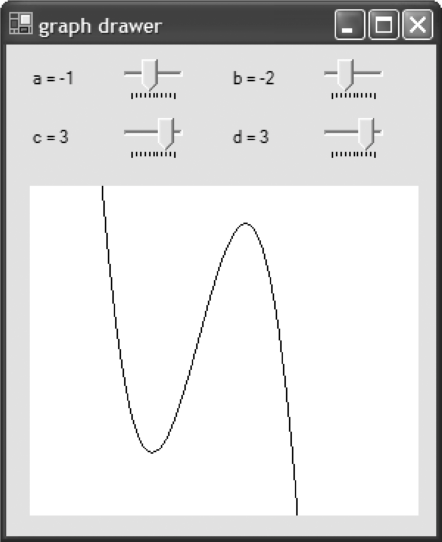
\includegraphics[width=8cm]{calculations_graph_screen}
			\caption{Screen of the graph drawer program, with cubic function displayed.}
			\label{fig:calculations_graph_screen}
		\end{figure}

		
		We must resolve several design issues. First we want to see the graph with the y-coordinate going up the screen, whereas y pixel coordinates measure downwards. We will distinguish between $x$ and its equivalent pixel coordinate \keyword{xPixel}, and between $y$ and \keyword{yPixel}.
		
		Next we have to ensure that the graph will fit conveniently within the picture box, that it is not too small to see or too big to fit. Solving this problem is called scaling. We will assume that the available area in a picture box is 200 pixels in the $x$ direction and 200 pixels in the $y$ direction. We will design the program to display $x$ and $y$ values in the range $\pm5.0$. So 1 unit of $x$ (or $y$) is 20 pixels.
		
		Finally, since we will be using \keyword{DrawLine} to draw the graph, we will have to draw a curved shape as a large number of small lines. We will move along the $x$ direction, one pixel at a time, drawing a line from the equivalent $y$-coordinate to the next. For each $x$ pixel, the program:
		\begin{enumerate}
			\item	calculates the $x$ value from the $x$ pixel value,
			\item	calculates the $y$ value, the value of the function,
			\item	calculates the $y$ pixel value from the $y$ value,
		\end{enumerate}
		using the following statements:
		\begin{lstlisting}
x = ScaleX(xPixel)
y = TheFunction(x)
yPixel = ScaleY(y)
		\end{lstlisting}
		The program then goes on to the next x pixel and again calculates the equivalent y pixel:
		\begin{lstlisting}
nextXPixel = xPixel + 1
nextX = ScaleX(nextXPixel)
nextY = TheFunction(nextX)
nextYPixel = ScaleY(nextY)
		\end{lstlisting}
		Finally the small section of the curve is drawn:
		\begin{lstlisting}
paper.DrawLine(myPen, xPixel, yPixel, nextXPixel, nextYPixel)
		\end{lstlisting}
		You will see that the program uses several private methods to help simplify the logic. Also just one method is used to handle the events from all the four track bars. Here is the complete code for this graph-drawing program.
		
		At class level are the variables:
		\begin{lstlisting}
Private a, b, c, d As Double
Private paper As Graphics
Private myPen As Pen = New Pen(Color.Black)
		\end{lstlisting}
Then the methods:
		\begin{lstlisting}
Private Sub TrackBar_Scroll( sender As System.Object,
		 e As System.EventArgs)
		Handles TrackBarA.Scroll,
			TrackBarB.Scroll,
			TrackBarC.Scroll,
			TrackBarD.Scroll
	DrawGraph()
End Sub
Private Sub DrawGraph()
	a = TrackBarA.Value
	LabelA.Text = "a = " & CStr(a)
	b = TrackBarB.Value
	LabelB.Text = "b = " & CStr(b)
	c = TrackBarC.Value
	LabelC.Text = "c = " & CStr(c)
	d = TrackBarD.Value
	LabelD.Text = "d = " & CStr(d)
	paper.Clear(Color.White)
	Draw()
End Sub
Private Sub Draw()
	Dim x, y, nextX, nextY As Double
	Dim xPixel, yPixel, nextXPixel, nextYPixel As Integer
	For xPixel = 0 To PictureBox1.Width
		x = ScaleX(xPixel)
		y = TheFunction(x)
		yPixel = ScaleY(y)
		nextXPixel = xPixel + 1
		nextX = ScaleX(nextXPixel)
		nextY = TheFunction(nextX)
		nextYPixel = ScaleY(nextY)
		paper.DrawLine(myPen, xPixel,
			yPixel, nextXPixel, nextYPixel)
	Next
End Sub
Private Function TheFunction( x As Double) As Double
	Return a * x * x * x + b * x * x + c * x + d
End Function
Private Function ScaleX( xPixel As Integer) As Double
	Dim xStart As Double = -5, xEnd As Double = 5
	Dim xScale As Double = PictureBox1.Width / (xEnd – xStart)
	Return (xPixel – (PictureBox1.Width / 2)) / xScale
End Function
Private Function ScaleY( y As Double) As Integer
	Dim yStart As Double = -5, yEnd As Double = 5
	Dim pixelCoord As Integer
	Dim yScale As Double = PictureBox1.Height / (yEnd – yStart)
	pixelCoord = CInt(-y * yScale) +
			CInt(PictureBox1.Height / 2)
	Return pixelCoord
End Function
		\end{lstlisting}
		If you run this program you can alter the track bar values to see the effect of changing the parameters. You can also draw quadratics (by making the value of coefficient a equal to zero) and straight lines, of course.


	\section{Exceptions}
		If you are reading this chapter for the first time, you should probably skip this section, because it deals with things that don't happen very often.
		
		When you write a program that does calculations, you have to watch out that you don't exceed the size of numbers that are allowed. It is not like doing a calculation on a piece of paper, where numbers can get as big as you like – it is more like using a calculator, which has a definite upper limit on the size of numbers that it will hold.
		
		So for example if you declare an \keyword{Integer}:
		\begin{lstlisting}
Dim number As Integer
		\end{lstlisting}
		you must be aware that the biggest number that can be held in an \keyword{Integer} is 2147483647. So if you write this:
		\begin{lstlisting}
number = 2147483647
number = number + 2147483647
		\end{lstlisting}
		the result of the addition cannot be accommodated as an \keyword{Integer} value. The program terminates and an error message is displayed. This is called \emph{overflow} and is one of a number of possible \emph{exceptions} that can arise as a program executes.
		
		Overflow can happen more subtly than this, particularly when a user enters data into a text box and its size is therefore unpredictable. For example, here is a simple program to calculate the area of a room in which overflow could occur:
		\begin{lstlisting}
Dim length, area As Integer
length = CInt(Textbox1.Text)
area = length * length
		\end{lstlisting}
		Situations that can lead to overflow are:
		\begin{itemize}
      \item adding two large numbers;
      \item subtracting a large positive number from a large negative number;
      \item dividing by a very small number;
      \item multiplying two large numbers.
				You can see that even with a simple calculation that looks harmless, vigilance is required. There are several ways to deal with an exception:
      \item Ignore it, hope it will not happen, and be prepared for the program to crash and/or give strange results when it does. This is OK for novice programs, but may be less than ideal for real programs designed to be robust.
			\item Allow the exception to arise but handle the exception by writing an exception handler as described later in \Cref{ch:exceptions}.
      \item Avoid it by writing in checks to ensure that such a situation is prevented. For example, in a program to calculate the area of a room, avoid overflow by checking the size of the data:
				\begin{lstlisting}
If length > 10000 Then
' take some action here
End If
				\end{lstlisting}
		\end{itemize}

		We have seen how overflow can happen when a program uses \keyword{Integer} values. We might expect the same thing to happen if \keyword{Double} values get too large – but it doesn't. Instead, if a value gets too large, the program keeps on going, and the value takes on a special value, one of NAN (Not A Number), positive infinity or minus infinity.


	\section{Programming principles}
		\begin{itemize}
      \item Many programs in science, engineering, mathematics and statistics employ lots of calculations. But even small programs that might not obviously need to do computations often use some arithmetic.
      \item The first and key step is deciding what types of variable to use to represent the data. The main choice is between \keyword{Integer} and \keyword{Double}.
      \item It is common to use iteration in numerical computation as the solution converges towards the answer. This involves a loop.
      \item The library of mathematical functions is invaluable in programs of this type.
      \item Exceptional situations, like overflow, can arise during calculations and should be anticipated if the program is to work robustly in all circumstances.
		\end{itemize}

				
	\section{Programming pitfalls}
		Exceptional situations such as trying to divide by zero can lead to strange results or else the program terminating. Make your programs robust.

		
	\section{Summary}
		\begin{itemize}
      \item Numbers can be represented as either \keyword{Integer} or \keyword{Double}. These provide different ranges and precision.
			\item A variable can be declared as \keyword{Const}. The value of such a variable cannot be changed when the program executes.
      \item Library functions provide the common mathematical functions, e.g. the sine of an angle.
      \item The programmer should be aware of exceptions that might arise during calculations 
		\end{itemize}

	\section{Exercises}
		\begin{EXE}
			\item	\name{Cost of phone call} A phone call costs 10 cents per minute. Write a program that inputs via text boxes the duration of a phone call, expressed in hours, minutes and seconds, and displays the cost of the phone call in cents.
			\item \name{Measurement conversion} Write a program to input a measurement via two text boxes expressed in feet and inches and convert the measurement to centimetres.
			There are 12 inches in a foot. One inch is 2.54 centimetres.
			\item	\name{Cash register} Write a program that represents a cash register. Amounts of money can be entered into a text box and are automatically added to the running total. The running total is displayed in another text box. A button allows the sum to be cleared (made zero).
			\item	\name{Sum of integers} The sum of the integers from 1 to $n$ is given by the formula:
				\begin{equation*}
					sum = n(n + 1)/2
				\end{equation*}
				Write a program that inputs a value for $n$ from a text box and calculates the sum two ways – first by using the formula and second by adding up the numbers using a loop.
			\item	\name{Random numbers} Random numbers are often used in computational and simulation programs, called Monte Carlo methods. The library class \keyword{Random} enables us to create a random number generator as follows:
				\begin{lstlisting}
Dim generator As Random = New Random()
				\end{lstlisting}
				This class has a method named \keyword{Next}, which returns a random number, an \keyword{Integer} in any range we choose (specified by the parameters). For example:
				\begin{lstlisting}
Dim number As Integer
number = generator.Next(1, 6)
				\end{lstlisting}
				Write a program to check out the random number generator method by asking it for 100 random numbers that have the value either 1 or 2. Count the number of values equal to 1 and those equal to 2. Provide a button that enables a further set of 100 values to be created.
			\item \name{Series for $e$} The value of $e^x$ can be calculated by summing the series:
				\begin{equation*}
					e^x = 1 + x + \frac{x^2}{2!} + \frac{x^3}{3!} + …
				\end{equation*}
				Write a program to input a value of x from a text box and calculate ex to a desired degree of accuracy. Check the value against the value obtained by referring to the constant \keyword{E} in the \keyword{Math} library.
			\item \name{Tax calculation} Write a program that carries out a tax calculation. The tax is zero on the first \$10 000, but is 33\% on any amount over that amount. Write the program to input a salary in dollars from a text box and calculate the tax payable. Watch out for errors when you perform the calculation – the answer needs to be accurate to the nearest cent!
			\item \name{Area of triangle} The area of a triangle with sides of length $a$, $b$, $c$ is:
				\begin{equation*}
					\text{area} = \sqrt{s (s-a) (s-b) (s-c)}
				\end{equation*}
				where
				\begin{equation*}
					s = (a + b + c)/2
				\end{equation*}
				Write a program that inputs the three values for the sides of a triangle from text boxes and uses this formula to calculate the area. Your program should first check that the three lengths specified do indeed form a triangle. So, for example, $a + b$ must be greater than $c$.
			\item	\name{Square root} The square root of a number can be calculated iteratively as shown below. Write a program to do this for a number input using a text box.
				\begin{itemize}
		      \item The first approximation to the square root of $x$ is $x/2$.
    		  \item Then successive approximations are given by the formula:
						\begin{equation*}
							\text{nextApproximation} = (\text{lastApproximation}^2 - x)/2 + \text{lastApproximation}
						\end{equation*}
				\end{itemize}
				Check the value against that obtained by using the library method \keyword{Sqrt}.
			\item	\name{Mathematical calculator} Write a program that acts as a mathematical calculator. It provides buttons with which to enter numbers, which are displayed like the display on a desk calculator. Buttons are also provided to carry out standard mathematical calculations like sine, cosine, natural logarithm and square root.
			\item \name{Interest calculator} Rewrite the calculation part of the program given above in the text so as to use an \keyword{Integer} number (instead of a \keyword{Double}) to represent an amount of money (expressed in cents).
			\item	\name{Graph drawer} Enhance the graph-drawing program in the program text so that it:
				\begin{itemize}
	      	\item draws the $x$- and $y$-axes;
  	  	  \item inputs the coefficients from text boxes instead of track bars (to give precision);
    		  \item inputs a horizontal and a vertical scaling (zoom) factor from track bars;
  	    	\item draws a second graph of the same function, but with different coefficients;
					\item draws the graphs of some other functions. One way to do this would be to rewrite the method \keyword{TheFunction}.
				\end{itemize}
			\item	\name{Numerical integration} Write a program that calculates the integral of a function $y$ using the 'trapezium rule'. The area under the graph of the function is divided into $n$ equal strips of width $d$. Then the area under the curve (the integral) is approximately the sum of all the (small) trapeziums:
				\begin{equation*}
					\text{area} \approx d(y_0 + 2y_1 + 2y_2 + . . . + 2y_{n-1} + y_n)/2
				\end{equation*}
				or:
				\begin{equation*}
					\text{area} = (\text{half the width of the strip}) × (\text{first} + \text{last} + \text{twice the sum of the others})
				\end{equation*}
				Use a function for which you know the answer, and experiment by using smaller and smaller values of $d$.
			\item	\name{Mandelbrot set} The Mandelbrot set (\Vref{fig:calculations_mandelbrot_screen}) is a famous and striking image produced by repeatedly evaluating a formula at each point in a two-dimensional space. Take a point, with coordinates $x_\text{start}$ and $y_\text{start}$. Then repeatedly calculate new values of $x$ and $y$ from the old values using the formulae:
				\begin{align*}
					x_\text{new} &= x_\text{old}^2 - y_\text{old}^2 - x_\text{start}\\
					y_\text{new} &= 2 x_\text{old} y_\text{old} - y_\text{start}
				\end{align*}
				The first values of $x_\text{old}$ and $y_\text{old}$ are $x_\text{start}$ and $y_\text{start}$. For each iteration, calculate $r = \sqrt{x_\text{new}^2 + y_\text{new}^2}$. Repeat until $r$ > 10 000 or 100 iterations, whichever comes first. 

				If $r$ is greater than 10 000, colour the pixel corresponding to this coordinate white, otherwise black.
				
				Repeat for all points with $x$ between -1.0 and +2.0 and $y$ in the range $\pm 2.0$.
				
				As the iteration proceeds, starting from particular values of $x_\text{start}$ and $y_\text{start}$, the value of $r$ sometimes remains reasonably small (around 1.0). For other values of $x_\text{start}$ and $y_\text{start}$, the value of $r$ quickly becomes very large and tends to shoot off to infinity.
				\begin{figure}[bth]
					\centering
					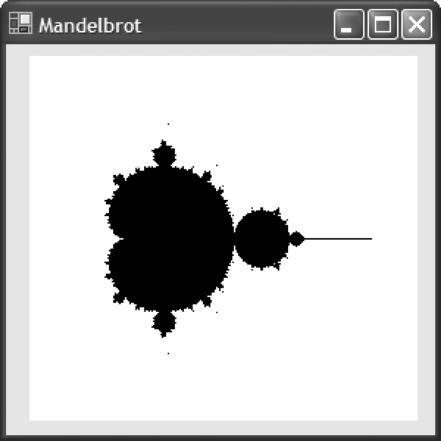
\includegraphics[width=8cm]{calculations_mandelbrot_screen}
					\caption{The Mandelbrot set.}
					\label{fig:calculations_mandelbrot_screen}
				\end{figure}
		\end{EXE}

		\begin{stab}
			\begin{enumChapter}
			\item
				\begin{lstlisting}
5E3
-0.56E-6
				\end{lstlisting}
			\item	
				\begin{lstlisting}
0.12
123,456.70
				\end{lstlisting}
			\item
				\begin{lstlisting}
Const lightSpeed As Double = 299792458
				\end{lstlisting}
		\end{enumChapter}
	 \end{stab}
